
The global ledger state is stored locally by each node in a key value pair database. Any performant database such as RockDb can be used to store the state data, however the data must be organised using a structure called a sparse Merkle tree. This structure allows the entire data state to be represented by a single hash, known as the root hash. Any changes to the data would result in a completely different root hash, therefore it can be used by nodes to verify that their dataset is the same as that of other nodes. Consequently, a node using an alternative storage organisation would be unable to interact with the network due to an inability to calculate the same root hash.\\

The sparse Merkle tree data structure allows for:

\begin{enumerate}
\item Persistent storage of the current and previous states of the ledger.
\item Efficient provision of proof that queried data exists, or importantly, does not exist in the ledger.\end{enumerate}

In addition to storing the global ledger state in a sparse Merkle tree, the smart contract KVM code and smart contract data are also stored using this data structure. This allows the root hash of both these data sets to be stored in the \textbf{storageRoot} and \textbf{codeHash} fields in the account state.  The use of the SMT for storing these data sets allows honest nodes to recognise and reject information that has been altered outside of the ledger cycle by malicious parties. \\

\subsubsection{Merkle Tree}

Each item of data being stored is represented as a leaf of the Merkle tree. The data in neighbouring leaves is hashed and concatenated and this value is used for the node one level above in the tree. Each node is stored in the database with its lookup key being the hash of its value. The nodes are themselves combined until a single hash has been obtained. This is the root hash and its value depends on every bit of data stored in the tree.\\

\begin{figure}[h]
  \centering
  \captionsetup{format=hang, font=footnotesize}
  \caption{A binary Merkle tree.}
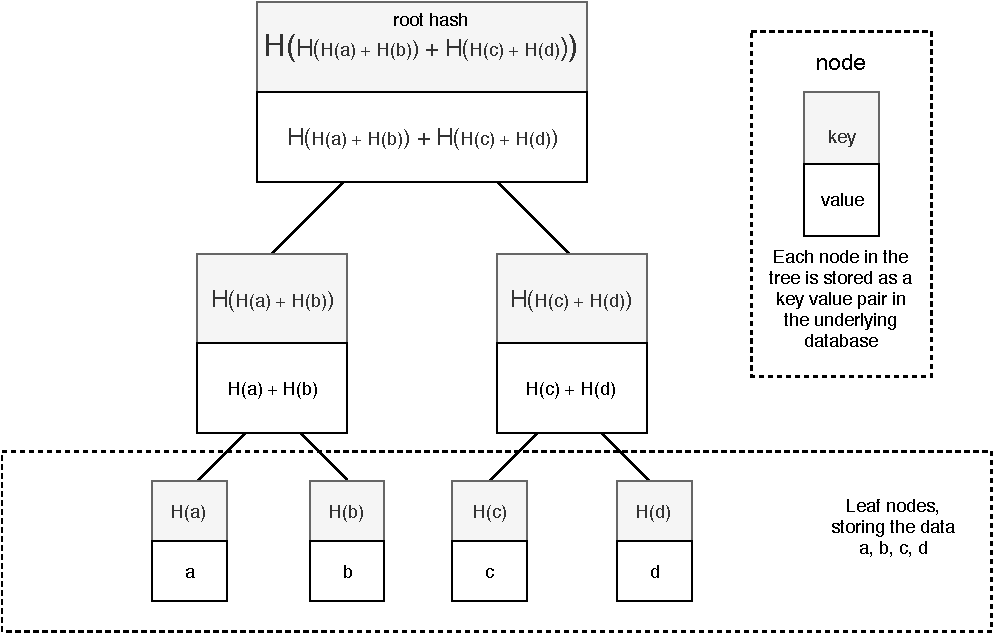
\includegraphics[scale=0.8]{merkle-tree}
\end{figure}

A binary tree is one in which the nodes can have only two children. Note that not all Merkle trees are binary trees. For example the nodes in a Modified Merkle Patricia tree can have up to 16 children.\\

When a data entry changes, every node above it in the tree must be recalculated. The hash of the data held by a node is used as its key in the database, therefore every recalculated node will constitute a new entry in the underlying database, rather than an existing entry that needs to be updated. This means that previous states of the tree are not overwritten, and all old data can be accessed using previous root hashes.\\

\subsubsection{Merkle Proof}

A client with knowledge of the current root hash of the state tree does not need to retrieve the complete set of data to verify the inclusion of a specific entry. Knowledge of each sibling hash along the path down to the entry being authenticated is sufficient to reconstruct the root hash. A client who is able to reconstruct the root hash from this data can be confident that the entry is contained in the data set. For example, in the diagram above, the inclusion of entry $\beta$ can be verified with just $\beta$, $H(\kappa)$, and $H(\lambda)+H(\sigma)$. \\

Though it is simple to prove inclusion of an item using a Merkle tree, proving that a particular item is \emph{not} included can be harder. This is because the item could exist at any of the leaf nodes.\\

\subsubsection{Sparse Merkle Tree}

The Sparse Merkle tree is a binary tree. The position of an entry in the sparse merkle tree is determined by its hash. For the ledger state, we use the hash of the account address to determine the index of the leaf node to hold the account data. This account index is used to determine the path from the root hash to the data entry, telling us which branch to follow as we progress down the tree. The account index is not equivalent to a key in the underlying database.\\

In a sparse tree a default value is used for leaves that do not yet contain data.\\

\begin{figure}[h]
  \centering
  \captionsetup{format=hang, font=footnotesize}
 \caption{A sparse Merkle tree, containing a single entry. The default values are represented by $\phi$.}
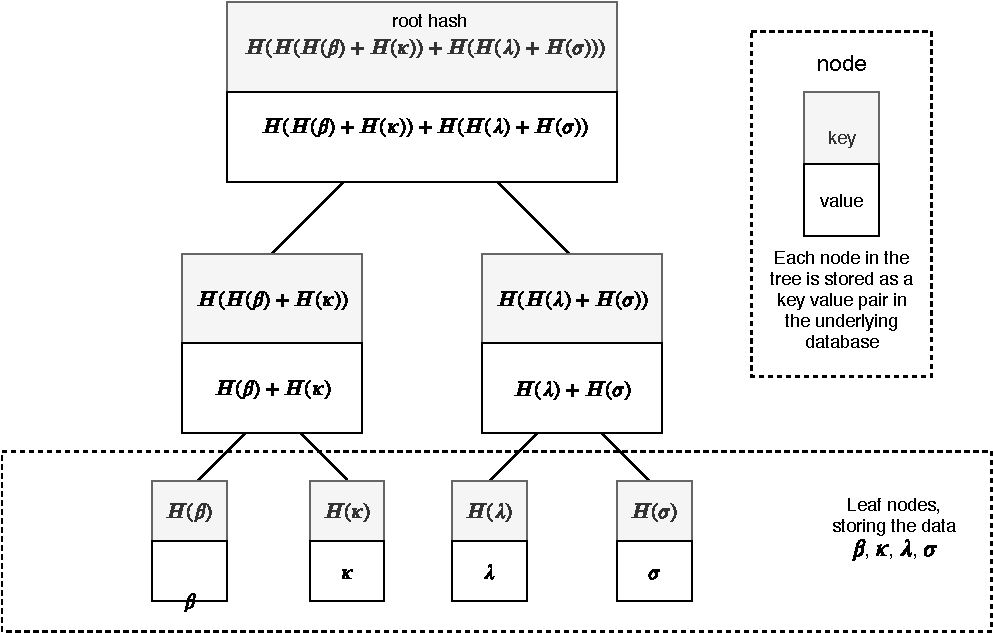
\includegraphics[scale=0.8]{sparse-merkle-tree}
\end{figure}

Since a data entry in a sparse Merkle tree can only exist in a specific location, proofs of non-inclusion are easy to provide; the proof that a key is not included in the tree is simply a proof that the value for the key is default.\\

A naive implementation would require a tree with a leaf for each possible index. Using the hash of the address as the index gives $2^{256}$ possible indices, too many to generate a full tree. However, non default entries will be uncommon compared to default entries; most of the nodes will therefore have default values that can be determined based on the height of the node. These values do not need to be stored more than once. For a branch containing only one non default entry, the entry can be stored in topmost node for that branch, providing further storage savings.\\
 
\subsubsection{Choice of Sparse Merkle Tree over the Modified Merkle Patricia Tree}

In a Patricia tree, each node can contain up to 16 children. As the sparse Merkle tree is a binary tree, it is simpler both to implement and to traverse the path to a leaf.  \\

For the Patricia tree, the Merkle proof is composed of all the nodes in the path. Since each node has 16 children the amount of data is larger and not as straightforward to verify as in a binary tree. Using a sparse Merkle tree gives us Merkle proofs which are small and easy to use.\\

